With the rise of social media services, more and more people share their opinions, feelings, experiences on the web. The roles of users shift from information consumers to information producers. To understand the attitudes and emotions behind these texts, sentiment analysis has become a popular research topic in recent years. 

Sentiment dictionaries tell machine how a writer or speaker may feel when using some term or phrase. They are important elements for several sentiment analysis approaches~\cite{Taboada:lexiconBased11, Rao:WWW14, Wen:AAAI14, Lee:IJCNLP2011}, but in Chinese, they are relatively scarce or non-public. As the result, it is helpful to collect the sentiment information in Chinese. However, there are two problems in collecting sentiment information. First, its coverage and quality highly affect the performance of sentiment analysis for texts, but collecting the information with high coverage, quality but low cost is challenging. The second problem is that the sentiments of several terms and phrases are context-dependent. How to define context, collect the sentiments on different contexts efficiently and decide which context and sentiment should be used to predict sentiments of texts are challenges.

For the first problem, several approaches~\cite{Strapparava:IREC04, Esuli:LREC06, Liu:IUI03, Cambria:AAAI10, Wu:TAAI11, Tsai:IEEE13, Wu:relSelect14} have used the external knowledge such as WordNet~\cite{Miller:WordNet95} and ConceptNet~\cite{Havasi:RANLP07,Speer:LREC12} to build sentiment dictionaries automatically. The relationship information in WordNet and ConceptNet is used to propagate sentiments from some seeds, which had been compiled manually. 

ConceptNet is a semantic network which represents knowledge into more computable representations. The nodes in ConceptNet are called {\it concepts} because the coverage of nodes contains not only lexical terms but also higher-order compound concepts, e.g., 'accomplish goal', 'leave behind'. A directed edge connecting two nodes is called {\it relation}, and is associated with one of the predefined types of labels to represent the semantic relationships between two {\it concepts} in real world, e.g., 'CapableOf', 'Causes'. The former {\it concept}, latter {\it concept} and their {\it relation} form an {\it assertion}, such as ``oven UsedFor cook", ``eat HasSubevent swallow". Because ConceptNet has large amount of {\it concepts} (In Chinese part~\cite{Kuo:HCOMP09,Kuo:FSS10}, there are at least 220000 {\it concepts}, still growing...), and its {\it concepts} have higher semantic meaning than traditional lexical terms, it is a good foundation to build a larger sentiment dictionary. In this paper, we collect sentiments based on {\it concepts} and the structure in Chinese ConceptNet.

However, previous propagation approaches in ConceptNet didn't deal with the issue that a {\it concept}'s neighbors may come from different scenarios. Take Figure~\ref{fig:noWork2} for example, previous approaches aggregate the sentiments from neighbors disregarding their different scenarios, and assign the aggregated sentiment to 'do not have to work'. 'do dot have to work' will propagate this sentiment to all its neighbors in the next iteration, which makes sentiments be propagated between different scenarios.

\begin{figure}[!t]
\centering
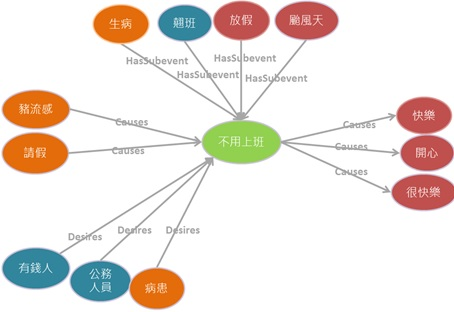
\includegraphics[width=2.5in]{fig/noWork2.jpg}
\caption{Neighbors of 'do not have to work' come from different scenarios.}
\label{fig:noWork2}
\end{figure}

The second problem is that each {\it concept} should be assigned different sentiments in different scenarios. For example, 'scream' is more possible to be negative when 'pervert' or 'cockroach' appears, but is more likely to be positive when 'idol' or 'win' appears. Previous approaches ~\cite{Xu:PACLIC10, Xu:COLING10, Rao:WWW14} use domain-specific corpus to modify sentiment value according to the corpus. However, hidden contextual information in Chinese ConceptNet is also abundant, like Figure~\ref{fig:noWork2}. If we could know which scenario an assertion belongs to, a {\it concept}'s sentiment in a scenario can be determined from its assertions which belongs to the scenario. 

To deal with the two problems, this paper develops a topic-aware propagation method for Chinese ConceptNet. We extract hidden contextual information by applying Latent Dirichlet Allocation~\cite{Blei:LDA03} to Chinese ConceptNet. The information divides Chinese ConceptNet into different topic layers where each topic is a distribution over concepts. Then, sentiment propagation can be performed on each topic layer. This not only avoids propagating sentiments between different scenarios but also generating sentiment on each topic for each concept. Then we present how to apply these topic-aware sentiment values of {\it concepts} to polarity classification for texts. Finally, two experiments are conducted. The first experiment use part of concepts to test the results of topic-insensitive and topic-aware propagation. It shows the effect of introducing topics to avoid propagation between different scenarios. The second experiment is conducting on the microblog dataset provided by the Chinese Microblog Sentiment Analysis Evaluation (CMSAE) task in the conference on Natural Language Processing \& Chinese Computing (NLP \& CC) 2013 \footnote{\url{http://tcci.ccf.org.cn/conference/2013/pages/page04_dg.html}}. The result show that compared with assigning a concept a fixed sentiment value, identifying its topic and select a proper sentiment value performs better.